\documentclass[11pt]{article}
\usepackage[MeX]{polski}
\usepackage{graphicx}
\title{Albert Einstein}
\author{Jan Dołkowski}
\date{20.01.2020}
\begin{document}
\maketitle
\newpage
\tableofcontents
\listoftables
\listoffigures
\newpage
\section{Wstęp}
\textbf{Albert Einstein} (ur. 14 marca 1879 w Ulm, zm. 18 kwietnia 1955 w Princeton) – fizyk teoretyczny i laureat Nagrody Nobla w dziedzinie fizyki w 1921 roku za „wkład do fizyki teoretycznej, zwłaszcza opis prawa efektu fotoelektrycznego”. Twórca szczególnej teorii względności i autor wynikającej z niej równoważności masy i energii, sformułowanej słynnym wzorem {\large $$E = mc^2$$} Twórca ogólnej teorii względności oraz opartych na niej pierwszych modeli kosmologicznych oraz przewidywań dotyczących fal grawitacyjnych. Współtwórca teorii fotonu i dualizmu korpuskularno-falowego światła, a przez to mechaniki kwantowej. Jednocześnie – czołowy krytyk jej najczęstszej, kopenhaskiej interpretacji i współautor paradoksu EPR. Odkrywca emisji wymuszonej, statystyki Bosego-Einsteina i możliwości istnienia kondensatu Bosego-Einsteina. Zwykle jest uznawany za niemieckiego fizyka żydowskiego pochodzenia; por. niżej. Einstein jest uważany za jednego z największych lub największego fizyka XX wieku, obok innych twórców mechaniki kwantowej – jak Paul Dirac, Werner Heisenberg czy Erwin Schrödinger – lub przed nimi. Jego ogólna teoria względności jest uważana za jeden z największych przełomów w fizyce XX wieku, obok wspomnianej teorii kwantów. Jednocześnie Einstein jest uznawany za jednego z największych fizyków w całej historii, obok Newtona, Maxwella czy Galileusza. W 1999 r. czasopismo naukowe Physics World w gronie 100 wiodących fizyków przeprowadziło ankietę. Jako największego fizyka wszech czasów wskazała właśnie Einsteina[1]. W 1999 r. Einstein był też uznany za człowieka stulecia według amerykańskiego tygodnika „Time”. Einstein opublikował ponad 450 prac, w tym ponad 300 naukowych. Wniósł też swój wkład do rozwoju filozofii nauki.
\newpage
\section{Życiorys}
\subsection{Dzieciństwo i rodzina}
Albert Einstein urodził się w piątek 14 marca 1879 r. o godzinie 11:30 w domu przy Bahnhofstrasse B nr 135 w mieście Ulm położonym w Wirtembergii na południu Niemiec. Jego matką była Paulina Einstein (z domu Koch), a ojcem – Hermann Einstein. Oboje byli Żydami. Hermann Einstein handlował pierzynami. Później jego brat Jacob namówił go do wspólnego założenia zakładu produkującego instalacje gazowe i wodno-kanalizacyjne. W 1881 r. cała rodzina przeniosła się do Monachium, gdzie powstał zakład. Tam też 18 listopada 1881 r. urodziła się Maria – jedyna siostra Einsteina.
Albert Einstein pierwszy raz zetknął się z nauką, gdy miał pięć lat. Jego ojciec pokazał mu kompas, którego działanie wywarło na nim „głębokie i trwałe wrażenie”. W tym czasie Einstein rozpoczął naukę w domu. Ponieważ jego matka była muzykiem, Albert w wieku sześciu lat zaczął uczyć się gry na skrzypcach. Lekcje gry pobierał do trzynastego roku życia. Grał do późnej starości, dopóki nie zaczęło mu to sprawiać zbyt dużego trudu\cite{Jeremy}.
\begin{figure}[ht]
\begin{center}
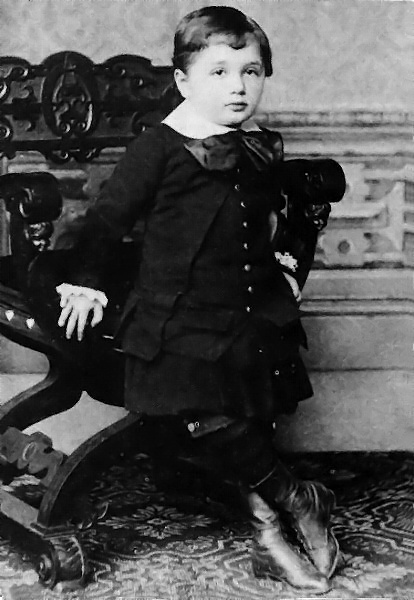
\includegraphics[width=6cm]{Albert_Einstein_at_the_age_of_three_(1882)}
\caption{zdjęcie młodego Ensteina}
\label{młody_einstain}
\end{center}
\end{figure}
\newpage
\subsection{Studia i małżeństwo}
W czasie studiów Einstein zakochał się z wzajemnością w Milevie Marić, co nie podobało się jego matce. W lipcu 1900 r. oboje zakochanych przystąpiło do zdawania egzaminów końcowych. Albert je zdał, w przeciwieństwie do Milevy. Wtedy też młody Einstein opublikował swoją pierwszą pracę naukową – dotyczyła zjawiska włoskowatości.
W 1901 r. Mileva zaszła w ciążę. Na czas porodu udała się do rodzinnej Serbii i urodziła tam córkę o imieniu Lise (zdrobniale Lieserl). Oddano ją po cichu do adopcji i jej dalsze losy są nieznane. Albert najprawdopodobniej nigdy jej nie zobaczył.
21 lutego 1901 r. Einstein przyjął obywatelstwo szwajcarskie. Mając już dyplom wykładowcy nauk ścisłych, zaczął szukać pracy. Starał się bezskutecznie o asystenturę u wykładającego w ETHZ Webera, a później u Hurwitza i Wilhelma Ostwalda. Dopiero w maju 1901 r. został zatrudniony na krótko jako zastępca nauczyciela w szkole średniej w Winterthur w Szwajcarii. W tym czasie zajmował się tam ruchem materii względem eteru i kinetyczną teorią gazów. Od października 1901 r. do stycznia 1902 r. uczył w prywatnej szkole w Schaffhausen, a równolegle pracował nad swoją pracą doktorską dotyczącą kinetycznej teorii gazów. W lutym 1902 r. przeprowadził się do Berna, gdyż spodziewał się dostać stałą pracę w Szwajcarskim Urzędzie Patentowym w Bernie. Utrzymywał się z udzielania korepetycji. W czerwcu został zatrudniony na okres próbny jako ekspert techniczny trzeciej klasy w urzędzie patentowym, a trzy miesiące później zatrudniono go na stałe.
10 października 1902 r., wskutek choroby serca, zmarł ojciec Einsteina. 6 stycznia 1903 r. Albert Einstein i Mileva Marić wzięli w Bernie ślub cywilny. 14 maja 1904 r. urodził się pierwszy syn Einsteina, Hans Albert, który później również został wybitnym uczonym. Kolejny syn, Eduard, urodził się 28 lipca 1910\cite{Denis}.
\newpage
\section{Nagroda Nobla}

\begin{table}
\caption{Wybrane nominacje do Nagrody Nobla}
\label{tab:nagrodaNobla}
\begin{center}
\begin{tabular}{|c|c|c|}
\hline rok & kategoria & liczba zgłaszających \\ \hline\hline
1912 & Fizyka Teoretyczna & 4\\
1913 & Fizyka Teoretyczna & 3\\
1920 & Fizyka Matematyczna & 8\\
1922 & Fizyka Matematyczna & 16\\ \hline
\end{tabular}
\end{center}
\end{table}
Albert Einstein był nominowany do Nagrody Nobla jedenastokrotnie – prawie corocznie w latach 1910–1922, z wyjątkiem 1911 i 1915. Jego kandydaturę zgłaszało 40 różnych naukowców – 12 z nich kilkukrotnie, np. Warburg (6 razy); Ostwald, Wien, Ehrenhaft, Naunyn, von Laue, E. Meyer, S. Meyer, Planck (po 3 razy); de Haas, Nordström, Hadamard (po 2 razy). Licząc osobno różne zgłoszenia przez tę samą osobę, Einstein otrzymał łącznie ponad 60 nominacji\cite{Jeremy}.
\newpage
\section{Stan Formalny}
\begin{itemize}
\item Do 17. roku życia był poddanym króla Wirtembergii.
\item 28 stycznia 1896 roku, na wniosek swojego ojca, został zwolniony z tego poddaństwa, dzięki czemu ojciec mógł złożyć prośbę o naturalizowanie syna jako obywatela Szwajcarii. Od tej daty do 21 marca 1901 Einstein pozostawał bezpaństwowcem.
\item 21 marca 1901 roku przyznano mu obywatelstwo Szwajcarii, a dokładnie miasta Zurych. Mieszkał nie tylko w Zurychu, ale także w Bernie wraz z żoną i dwoma synami. W cudownym roku 1905, kiedy opublikował szczególną teorię względności i inne przełomowe prace, był więc formalnie Szwajcarem. Z obywatelstwa Szwajcarii nigdy nie zrezygnował.
\item Od 1 kwietnia 1911 roku do 30 września 1912 roku, w związku z objęciem katedry fizyki teoretycznej na Uniwersytecie w Pradze, stał się poddanym cesarza Austrii, nadal pozostając jednocześnie obywatelem Szwajcarii.
\item 1 października 1940 roku złożył przysięgę na konstytucję i został obywatelem Stanów Zjednoczonych, pozostając aż do śmierci nadal również obywatelem Szwajcarii.
\end{itemize}
\vspace{1.2cm}
\begin{quotation}
\textit{"Jeżeli teoria względności okaże się prawdziwa, to Niemcy nazwą mnie wielkim Niemcem, Szwajcarzy – Szwajcarem, a Francuzi – wielkim uczonym. Jeżeli natomiast teoria względności okaże się błędna, wtedy Francuzi nazwą mnie Szwajcarem, Szwajcarzy – Niemcem, a Niemcy – Żydem."}\\
\begin{flushright}
Albert Einstein
\end{flushright}
\end{quotation}
\newpage
\section{Inne znane wzory}
$$R_{\mu \nu} - {1 \over 2}g_{\mu \nu}\,R + g_{\mu \nu} \Lambda = 
{8 \pi G \over c^4} T_{\mu \nu}$$\\To równanie jest również znane jako \textit{Równanie Einstaina}\\
\\$R_{\mu \nu}$ - tensor krzywizny Ricciego\\
$R$ - skala krzywizny Ricciego\\
$g_{\mu \nu}$ - tensor metryczny\\
$\Lambda$ - stała kosmologiczna\\
$T_{\mu \nu}$ - tensor energii-pędu\\
$\pi$ - liczba pi\\
$c$ - prędkość światła\\
$G$ - stała grawitacyjna
\begin{figure}[ht]
\begin{center}
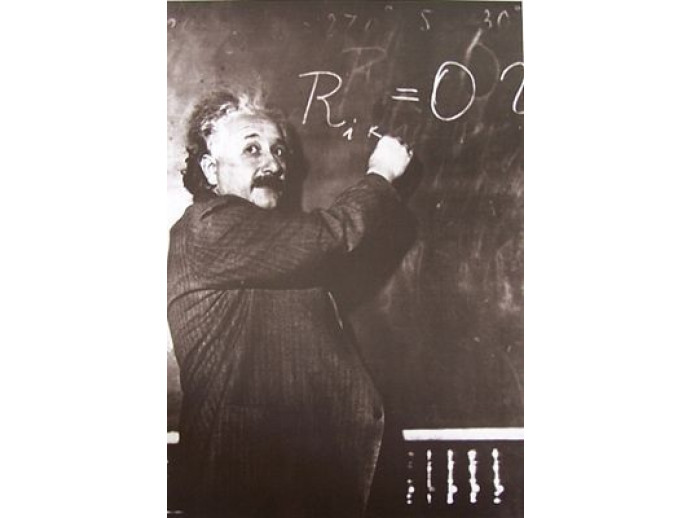
\includegraphics[width=11cm]{122404_1}
\caption{Einstain przy tablicy}
\label{einstain_tablica}
\end{center}
\end{figure}
\newpage
\begin{thebibliography}{9}
\bibitem{Denis}
Denis Brian,
\emph{Einstein: nowe, udostępnione w ostatnich latach dokumenty z Archiwum Einsteina.}
Warszawa: Wydawnictwo „Amber”, 1997.
\bibitem{Jeremy}
Jeremy Bernstein, \emph{Albert Einstein i granice fizyki.} Jarosław Włodarczyk (tłum.). Warszawa: Świat Książki, 2008.
\end{thebibliography}
\end{document}